\chapter{PDFBox}
    Le site web comprend une partie permettant aux éleves de consulter des cours 
en ligne, par les conférenciers soit en récupérant des pdf ou alors en visionnant
des "diapositives". Ces dernières correspondent à des pages de fichiers pdf qui
ont été au préalable convertit en image. 

    Cela a été possible en utilisant un projet open source PDFBox \cite{pdfbox}.
\newline
\newline

    \begin{figure}[h]
        \begin{center}
            
\includegraphics[scale=0.6]{PDFBox.png} 
        \end{center}

        \caption{Logo PDFBox}
        \label{Logo PDFBox}
    \end{figure}

\newpage



	\section{Présentation du projet PDFBox}
	PDFBox est une librairie open source codée en java, permettant de manipuler 
des documents pdf. Elle permet la création de manipuler les fichiers PDF de 
nombreuses façon.

	PDFBox est sous license Apache License v2.0, ce qui en fait un lobiciel libre 
et open source.

	Principales fonctionnalités:
	\begin{itemize}
		%expliquer pk difficile de differencier paragraphe si vraiment necessaire au rapport
		\item Extraction de texte.
		      Cette fonction est toujours au stade de devloppement car il est difficile de 
              différencier deux paragraphes différents dans un fichier pdf (la position 
              du texte est donnée par des positions absolue, ce qui permet de disposer 
              le texte exactement la où on le souhaite).  
		\item Fusion de documents PDF. 
		\item Encrypter/Décrypter.
		\item Créer un PDF depuis un fichier texte.
		\item Création d'images à partir d'un document PDF. C'est ce qui va 
              principalement nous intérésser. C'est cette dernière qui servira à 
              fournir les diapositives que les élèves pourront consulter à partir 
              du site web.
		\item Imprimer un PDF.
	\end{itemize}

		Il faut savoir que la fonction convertissant un pdf en images est encore
    au stade de développement. Ce qui veut dire que  les fonctionnalités ne sont 
    pas encore toutes implémentées ou encore que certains bugs subsistent encore.

        Ci-dessous nous allons expliquer les problèmes que nous avons rencontrés,
    ainsi que la manière dont nous avons résolus chacun d'entre-eux.

        Avant toute chose, il est important de noter que la résolution à ceux-ci
    à été possible grâce à la documentation de PDFBox et à celle de la classe 
    java.awt.Font ainsi qu'au débugueur inclus dans l'environnement de dévelopement 
    Eclipse.


	\section{MediaBox et CropBox}
        Lors de nos tests, nous nous sommes rendues compte qu'il pouvait y 
    avoir un problème de conversion avec un fichier pdf contenant à la fois une 
    "cropbox" et une "mediabox". Il faut savoir que lors de la visualisation d'un 
    document pdf, par défaut, on ne voit que la partie que l'auteur veut que l'on 
    voit. Ce procédé est par exemple utilisé dans les imprimeries. 

		\begin{itemize}
			\item La cropbox correspond  à la partie visible par tous du document, 
                  c'est celle qui est destinée à être vue.
			\item La mediabox comprend la cropbox et correspond à la totalité 
                  réelle du document et non pas seulement à la partie visible 
                  lors de la lecture du fichier avec Adobe Reader par exemple. 
		\end{itemize}

        %TODO: Image contenant cropbox et mediabox 
    
     \begin{figure}[h]
            \begin{center}
            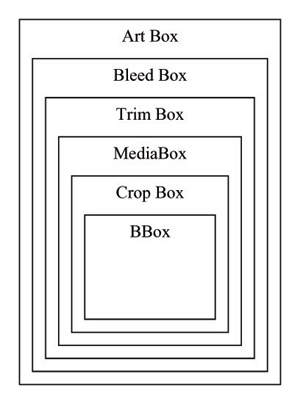
\includegraphics[scale=0.6]{crop_media_box.jpg} 
            \end{center}
            \caption{hiérarchie des différentes "box"}
            \label{hiérarchie des différentes "box" }
     \end{figure}

	        Ce premier problème se rapporte au fait de ne pas pouvoir convertir
        une page en entier si une cropbox était spécifiée (la médiabox l'est 
        obligatoirement elle). Pour cela, il a fallut envoyer les bonnes dimensions 
        de pages à chaque fois qu'une image est crée, et cela sans utiliser la fonction
        getcropbox retournant un objet de type PDRectangle et qui ne fonctionne 
        pas correctement (lance un null pointeur exception). On a donc changé le
        code pour faire appel à la fonction findcropbox() qui elle fonctionne 
        correctement.


	%TODO: Dire quel fichier et quelles lignes on été modifiés


    \lstset{language=Java}
	\begin{lstlisting} 
private static void changeCropBoxes(PDDocument document,float a, float b, float c,float d)
{
	List <PDPage> pages = document.getDocumentCatalog().getAllPages();
	for( int i = 0; i < pages.size(); i++ )
	{
        System.out.println("resizing page");
        PDPage page = (PDPage)pages.get( i );
        PDRectangle rectangle = new PDRectangle();
        rectangle = page.getMediaBox();
        a=0;
        rectangle.setLowerLeftY(a);
        rectangle.setLowerLeftY(b);
        rectangle.setUpperRightX(c);
        rectangle.setUpperRightY(d);

        page.setMediaBox(rectangle);
        page.setCropBox(rectangle);
	 }
}
 \end{lstlisting}

        Une fois que les dimensions recherchées sont récuperées, on les affectes
    aux pages du document PDF l'on veut convertir. Ainsi on obtient bien les bonnes 
    dimensions de pages.



    \section{Polices embarquées}
        Il faut savoir que suivant les softwares employés pour créer les PDF et
    les polices utilisées, il est possible de ces dernières soient directement
    inclues dans le fichier final. Cela est autorisé par la norme ISO régissant 
    ce type de fichier. Or en n interne, la gestion des polices est faites via 
    classe "java.awt.Font". Et malheuresement, cette dernière nécessite de travailler
    avec des polices complètes.

        Il arrive donc que suivant les fichiers à transformer en images, si la police 
    est contenue dedans, le resultats soit illisible, dû à la confusion par rapport
    au caractère manquant.

        %TODO: Image de diapositive erronée.

        Comme mentionnée précédemment, certains fichiers PDF, peuvent contenir eux 
    même la définition ainsi que les glyphes correspondants aux caractères utilisées dans 
    le document. Cependant, si ces dernières ne sont pas complètes, il subsistait
    quelques erreurs.

        Nous avons essayer de modifier nous même les polices incriminées mais 
    sans résultats probants. Nous avons donc patché le code une deuxième fois 
    en donnant la police système si le document en utilisait une interne.

        De ce fait tous les documents se verront ecris avec cette police mais 
    on garde l'avantage de garder partiellement le style d'écriture 
    (soulignement, couleur, taille).




%TODO: Donner les diffs en annexe



